\documentclass[a4paper,12pt]{article}
\usepackage{HomeWorkTemplate}
\usepackage{circuitikz}
\usepackage[shortlabels]{enumitem}
\usepackage{float}
\usepackage{hyperref}
\usepackage{tikz}
\usepackage{amsmath}
\usepackage{amssymb}
\usepackage{tcolorbox}
\usepackage{xepersian}
\settextfont{XB Niloofar}
\usetikzlibrary{arrows,automata}
\usetikzlibrary{circuits.logic.US}
\usepackage{changepage}
\newcounter{problemcounter}
\newcounter{subproblemcounter}
\setcounter{problemcounter}{1}
\setcounter{subproblemcounter}{1}
\newcommand{\problem}[1]
{
	\subsection*{
		پرسش
		\arabic{problemcounter} 
		\stepcounter{problemcounter}
		\setcounter{subproblemcounter}{1}
		#1
	}
}
\newcommand{\subproblem}{
	\textbf{\harfi{subproblemcounter})}\stepcounter{subproblemcounter}
}


\begin{document}
\handout
{آز طراحی سیستم‌های دیجیتال}
{دکتر سیاوش بیات سرمدی}
{نیم‌سال اول 1400\lr{-}1401}
{اطلاعیه}
{پرهام چاوشیان}
{98100118}
 {گزارش آزمایش پنجم}
{خانم زینب رشیدی}
مطابق با دستور کار هدف ساخت یه ماژول ضرب‌کننده $Booth$ با قابلیت چند شیفت در یک کلاک، مطابق با معماری گفته شده است. ماژول‌ها را شرح می‌دهیم:\\
\textbf{ماژول $shift\_countl_finder$} :
این ماژول کمک می‌کند تا بتوانیم در یک کلاک چندین شیفت بدهیم، تعداد شیفت مورد نیاز را، بر اساس تعداد بیت‌های یکسانی که کنار هم ظاهر شده‌اند به دست میآورد و در خروجی‌اش قرار می‌دهد.\\
\textbf{ماژول $control\_unit$} :
این ماژول باتوجه به وضعیت قبلی مدار، و همچنین گرفتن بیت‌ها
$Q_n$
و
$Q_{n\,+\,1}$
تعیین می‌کند که مدار باید در چه وضعیتی قرار گیرد و چه عملیاتی انجام شود.\\
\textbf{ماژول $datapath$} :
عملیاتی که باید انجام شود را در ورودی دریافت می‌کند و عملیات را انجام می‌دهد. وقتی کار نمام شد خروجی $done$ را یک می‌کند، همچنین حاصلضرب را در خروجی‌اش قرار می‌دهد.\\
\textbf{ماژول $Booth$} :
دو ماژول قبلی را به یکدیگر متصل کرده، و مدار را کامل می‌کند.\\
نتایج شبیه‌سازی نیز در ادامه آمده است، دقت کنید که خروجی تنها در پالس ساعتی که خروجی $done$ برابر 1 شده است، معتبر است. (در صورت نیاز تصاویر به طور جداگانه نیز پیوست شده اند):
\begin{figure}[H]
 \centering
  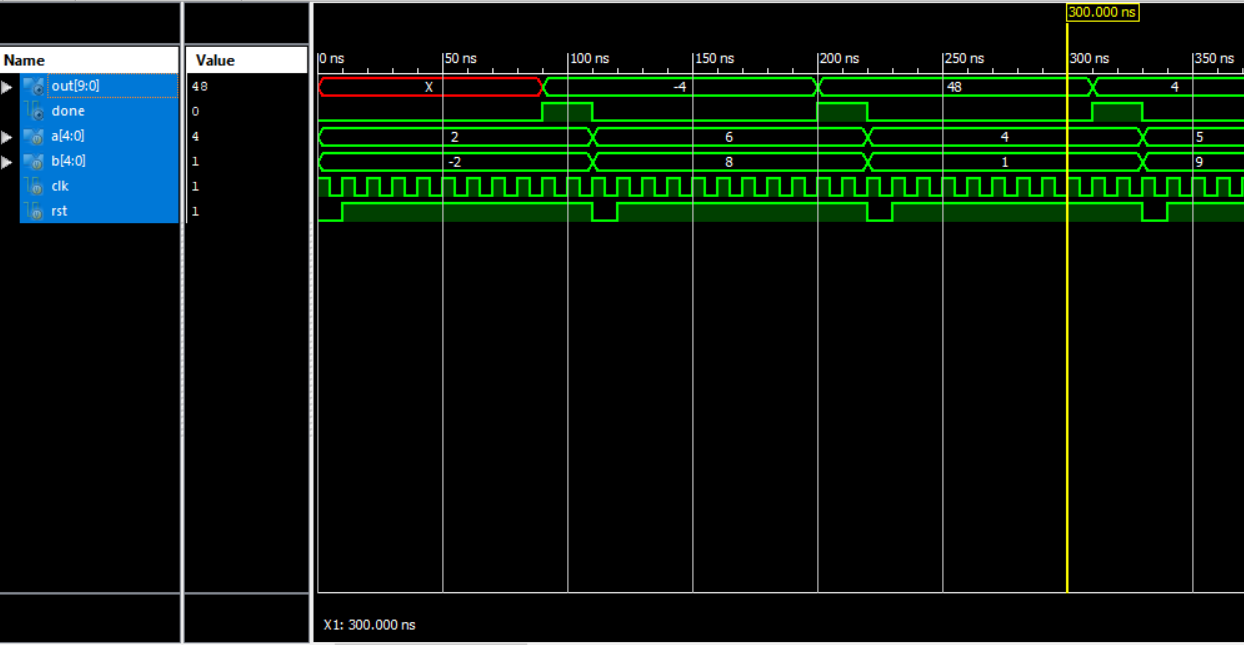
\includegraphics[width=0.8\linewidth]{s1}
\end{figure}
\end{document}